%\documentclass[11pt]{book}
%
%\setlength{\parindent}{0pt}
%\setlength{\parskip}{8pt}
%
%\usepackage{amsmath}
%\usepackage{amssymb}
%\usepackage{hyperref}
%\usepackage{cleveref}
%
%\renewcommand*{\thefootnote}{\fnsymbol{footnote}}
%
%\setcounter{chapter}{3}
%
%\begin{document}
%
%\section*{A Levelized Comparison of \\ Pulsed and Steady-State Tokamaks}
%
%\let\cleardoublepage\relax \tableofcontents \newpage

\chapter{Designing a Pulsed Tokamak}

\label{chapter:pulsed}

Pulsed tokamaks are the flagship of the European fusion \added{reactor design} effort. As such, this paper's model will now be generalized to accommodate this mode of operation. Fundamentally, this involves transforming current balance into flux balance -- adding inductive (pulsed) sources to stand alongside the LHCD (steady-state) ones.

The first step in generalizing current balance will be understanding the problem from a basic electrical engineering perspective -- i.e.\ with circuit analysis. The resulting equation will then be transformed into the flux balance seen in other models from the literature. All that will need to be done then is solving the problem for plasma current ($I_P$) and simplifying it for various situations -- e.g.\ steady-state operation.

\added{This generalized plasma current will then be found to be a function of the other dynamic variables (i.e.\ $R_0$, $B_0$, and $\overline T$). This, of course, is more difficult to handle computationally than the steady current, which only directly depended on temperature ($\overline T$). Discussion about solving this new root solving problem will be the topic of the next chapter.}

\section{Modeling Plasmas as Circuits}

Although it may have been lost along the way, what makes plasmas so interesting and versatile -- in comparison to gases -- is their ability to respond to electric and magnetic fields. It seems natural then to model plasma current from a circuits perspective (i.e.\ with resistors, voltage sources, and inductors). By name, this circuit is referred to as a transformer where: the plasma is the secondary and the yet-to-be discussed central solenoid (of the tokamak) is the primary.

The first step in deriving a current equation is to determine the circuit equations that govern pulsed operation in a tokamak. This will be done in two steps. First, we will draw a circuit diagram and write the equations that describe it. Next, we will use a simple schematic for how current evolves in a transformer to boil the resulting differential equations into simple algebraic ones -- as is the hallmark of our model.

\subsection{Drawing the Circuit Diagram}

Understanding a circuit always starts with drawing a simple diagram, see \cref{fig:circuit_diagram}. This figure depicts the transformer governing pulsed reactor. The left sub-circuit is the transformer's primary -- the central solenoid component of the tokamak that provides most of the inductive current. Whereas, the right sub-circuit is the plasma acting as the transformer's secondary. The central solenoid, here, is then a coiled metal structure that fits within the inner ring of the doughnut. For now, every other flux source (besides this central solenoid) is neglected.

\begin{figure}
\centering
\begin{circuitikz}
\draw (-1, 2) to [L,l_=$L_1$] (-1, -2) to (-5.5,-2) to [V,l=$V_1$, invert] (-5.5,2) to [short, i_=$I_1$] (-1,2);
\draw (+1,2) to [short, i_<=$I_2$]  (+5.5,2) to [R=$R_2$] (+5.5,-2) to (+1, -2) to [L,l_=$L_2$, invert] (+1, 2);
\draw (0, 1.25) node {$\bold{M}$};
\draw (+0.1, -0.6) to (+0.1, +0.6);
\draw (-0.1, -0.6) to (-0.1, +0.6);
\end{circuitikz}

\caption{A Simple Plasma Transformer Description} ~\\
\added{\small A plasma transformer consists of a solenoid primary (left) and a plasma secondary (right). They are connected by their mutual inductance, M. Note that the two currents -- $I_1$ and $I_2$ -- travel in opposite directions. }
\label{fig:circuit_diagram}
\end{figure}

\replaced{This is described by the standard circuits involving voltage sources, resistors, and inductors:}{Hopefully without scaring the reader too much, the circuit equations -- when only modeling voltage sources, resistors, and inductors -- are described by:}
\begin{equation}
	V_i = \sum_j^n \frac{d}{dt} \left( M_{ij} I_j \right) + I_i R_i \ \, , \ \ \ \ \forall \, i = 1,2,..,n
\end{equation}

Without going into the inductances (M) and resistances (R), the variable $n$ is the number of sub-circuits, here being 2. Whereas, the variables $i$ and $j$ are the indices of sub-circuits (i.e.\ 1 for the primary, 2 for the secondary). For illustrative purposes, this would boil down to the following relation for a battery attached to a lightbulb:
\begin{equation}
	V = I R
\end{equation}
Back to the transformer diagram, the equations for the two subcircuits can be expanded and greatly simplified. Besides ignoring every inductive source other than the central solenoid, the next powerful assumption is treating the solenoid as a superconductor (i.e.\ with negligible resistance). Lastly, the inductances between components and themselves are held constant -- independent of time. This allows the coupled transformer equations to be written as:
\begin{align}
	\label{eq:circ1}
	V_1 = L_1 \dot I_1 - M \dot I_2 \\
	\label{eq:circ2}
	-I_2 R_P = L_2 \dot I_2 - M \dot I_1
\end{align}
With $I_1$ and $I_2$ going in opposite directions. Note, here, that the subscript on M has been dropped, as there are only two components. This was done in conjunction to adding internal (self-)inductance terms. Mathematically, the mapping between variables is:
\begin{equation}
	M = M_{12} = M_{21}
\end{equation}
\begin{gather}
	L_1 = M_{11} \\
	L_2 = M_{22}
\end{gather}
Repeated, the one subscript represents the primary -- the central solenoid -- and the two stands for the plasma as the transformer's secondary. Exact definitions for the inductances will be put off till the end of the next subsection.

\subsection{Plotting Pulse Profiles}

Up until now, little has been discussed that has a time dependence. For steady-state tokamaks, this did not occur because it is an extreme case where pulses \replaced{could last weeks or months.}{basically last the duration of the machine's lifespan (i.e.\ around 50 years).} By definition, though, a pulsed machine has pulses -- with around ten scheduled per day.\cite{ac_pulses} For this reason, a fusion pulse is now investigated in detail.

Transformer pulses between the central solenoid and the plasma occur on the timescale of hours. \added{During this time, a plasma is brought up to some quasi-steady-state current ($I_P^*$) for \replaced{several}{around an} hour and then ramped back down using the available flux in the solenoid (measured in volt-seconds).} For clarity, each pulse is subdivided into four phases: ramp-up, flattop, ramp-down, and dwell. Pictorially represented in \cref{fig:circuit_profiles}, these divisions allow a simple scheme for transforming the coupled circuit differential equations -- from \cref{eq:circ1,eq:circ2} -- into simple algebraic formulas.

Along the way, we will approximate derivatives with linear piecewise functions. Using $t_i$ to represent the initial time and $t_f$ as the final one, these can be written as:

\begin{equation}
	\dot I = \frac{ I(t_f) - I(t_i) }{t_f - t_i}
\end{equation}

\newpage

\begin{figure}[b!]
\centering
\begin{adjustbox}{width=0.85\textwidth}
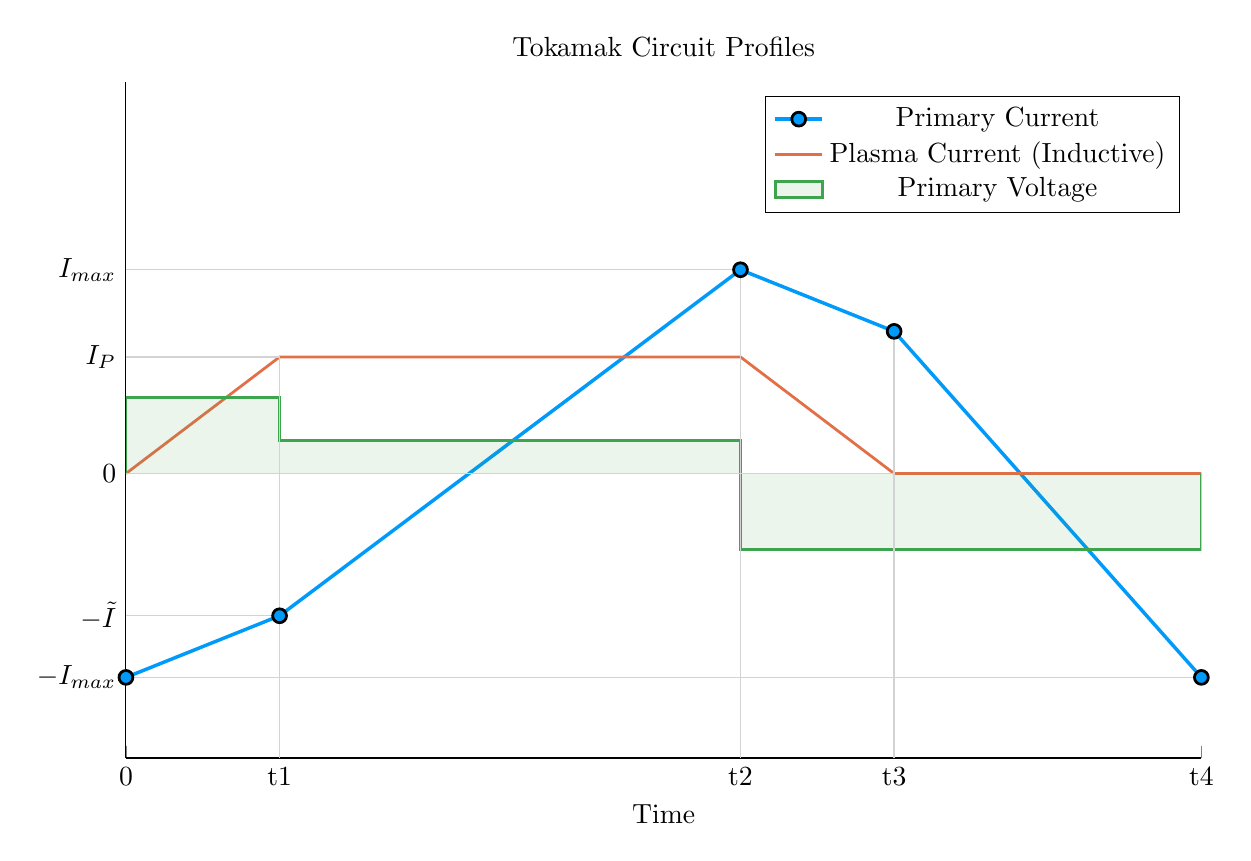
\begin{tikzpicture}[]
\begin{axis}[height = {101.6mm}, ylabel = {}, title = {Tokamak Circuit Profiles}, xmin = {0}, xmax = {7}, ymax = {4.125}, xlabel = {Time}, unbounded coords=jump,scaled x ticks = false,xticklabel style={rotate = 0},xmajorgrids = false,xtick = {0,1,4,5,7},xticklabels = {0,t1,t2,t3,t4},xtick align = inside,axis lines* = left,scaled y ticks = false,yticklabel style={rotate = 0},ymajorgrids = false,ytick = {0.0,-2.15,2.15,1.23,-1.5},yticklabels = {0,${-I_{max}}$,$I_{max}$,$I_P$,${-\tilde{I}}$},ytick align = inside,axis lines* = left,    xshift = 0.0mm,
    yshift = 0.0mm,
    axis background/.style={fill={rgb,1:red,1.00000000;green,1.00000000;blue,1.00000000}}
, ymin = {-3}, width = {152.4mm}]\addplot+ [color = {rgb,1:red,0.00000000;green,0.60560316;blue,0.97868012},
draw opacity=1.0,
line width=1.25,
solid,mark = *,
mark size = 2.5,
mark options = {
    color = {rgb,1:red,0.00000000;green,0.00000000;blue,0.00000000}, draw opacity = 1.0,
    fill = {rgb,1:red,0.00000000;green,0.60560316;blue,0.97868012}, fill opacity = 1.0,
    line width = 1,
    rotate = 0,
    solid
}]coordinates {
(0.0, -2.15)
(1.0, -1.5)
(4.0, 2.15)
(5.0, 1.5)
(7.0, -2.15)
};
\addlegendentry{Primary Current}
\addplot+ [color = {rgb,1:red,0.88887350;green,0.43564919;blue,0.27812294},
draw opacity=1.0,
line width=1,
solid,mark = none,
mark size = 2.0,
mark options = {
    color = {rgb,1:red,0.00000000;green,0.00000000;blue,0.00000000}, draw opacity = 1.0,
    fill = {rgb,1:red,0.88887350;green,0.43564919;blue,0.27812294}, fill opacity = 1.0,
    line width = 1,
    rotate = 0,
    solid
}]coordinates {
(0.0, 0.0)
(1.0, 1.23)
(4.0, 1.23)
(5.0, 0.0)
(7.0, 0.0)
};
\addlegendentry{Plasma Current (Inductive)}
\addplot+ [color = {rgb,1:red,0.24222430;green,0.64327509;blue,0.30444865},
draw opacity=1.0,
line width=1,
solid,mark = none,
mark size = 2.0,
mark options = {
    color = {rgb,1:red,0.00000000;green,0.00000000;blue,0.00000000}, draw opacity = 1.0,
    fill = {rgb,1:red,0.24222430;green,0.64327509;blue,0.30444865}, fill opacity = 1.0,
    line width = 1,
    rotate = 0,
    solid
},fill = {rgb,1:red,0.24222430;green,0.64327509;blue,0.30444865}, fill opacity=0.1,area legend]coordinates {
(0.0, 0.0)
(0.0, 0.8)
(1.0, 0.8)
(1.0, 0.35)
(4.0, 0.35)
(4.0, 0.0)
(NaN, NaN)
(4.0, 0.0)
(4.0, -0.8)
(7.0, -0.8)
(7.0, 0.0)
};
\addlegendentry{Primary Voltage}
\addplot+ [color = {rgb,1:red,0.82745098;green,0.82745098;blue,0.82745098},
draw opacity=1.0,
line width=0.5,
solid,mark = none,
mark size = 2.0,
mark options = {
    color = {rgb,1:red,0.00000000;green,0.00000000;blue,0.00000000}, draw opacity = 1.0,
    fill = {rgb,1:red,0.76444018;green,0.44411178;blue,0.82429754}, fill opacity = 1.0,
    line width = 1,
    rotate = 0,
    solid
},forget plot]coordinates {
(1.0, -4.25)
(1.0, 1.23)
(NaN, NaN)
(4.0, -4.25)
(4.0, 2.15)
(NaN, NaN)
(5.0, -4.25)
(5.0, 1.5)
(NaN, NaN)
(0.0, 1.23)
(1.0, 1.23)
(NaN, NaN)
(0.0, 2.15)
(4.0, 2.15)
(NaN, NaN)
(0.0, -1.5)
(1.0, -1.5)
(NaN, NaN)
(0.0, 0.0)
(5.0, 0.0)
(NaN, NaN)
(0.0, -2.15)
(7.0, -2.15)
};
\end{axis}

\end{tikzpicture}

\end{adjustbox}

\caption{Time Evolution of Circuit Profiles}
\label{fig:circuit_profiles} ~\\
\small{A circuit pulse involves four phases: (1) Ramp-Up, (2) Flattop, (3) Ramp-Down, and (4) Dwell. In reality, flattop can last more than 90\% of the pulse.\cite{inputfile} This makes the slope of the primary current during this phase much shallower than shown. } ~ \\ ~ \\ ~ \\
\end{figure}

In tabular form, the data from \cref{fig:circuit_profiles} can be written in this piecewise fashion as:

\begin{table}[h!]
\centering
\caption{Piecewise Linear Scheme for Pulsed Operation}
\hfill
\begin{subtable}[t]{0.4\textwidth}
\centering
\caption{Currents} ~\\
\begin{tabular}{ c|c|c }

\textbf{Time} & {$\bold{I_1}$} & {$\bold{I_2}$} \\
\hline
0 & $-I_{max}$ & 0 \\
t1 & $-\tilde I \ \ \ \,\, $ & $I_P^{\,*} $ \\
t2 & $+I_{max}$ & $I_P^{\,*}$ \\
t3 & $+\tilde I \ \ \ \,\, $ & 0 \\
t4 & $-I_{max}$ & 0 \\
\end{tabular}
\end{subtable}
\hfill
\begin{subtable}[t]{0.5\textwidth}
\centering
\caption{Voltage} ~\\
\begin{tabular}{ c|c|c|c }
\textbf{Phase} & $\bold{t_i}$ & $\bold{t_f}$ & $\bold{V_1}$ \\
\hline
Ramp-Up & 0 & $t_1$ & $+V_{max}$ \\
Flattop & $t_1$ & $t_2$ & $+ \tilde V$ \ \,\,\, \\
Ramp-Down & $t_2$ & $t_3$ & ${-V}_{max}$ \\
Dwell & $t_3$ & $t_4$ & ${-V}_{max}$ \\
\end{tabular}
\end{subtable}
\hfill
\hfill
\end{table}

\added{The exact definitions for the plasma's inductive current ($I_P^*$) and the maximum voltage in the central solenoid ($V_{max}$) will be put off until the end of the section.}

\newpage

\subsubsection{The Ramp-Up Phase -- RU}

The first phase in every plasma pulse is the ramp-up. During ramp-up, the central solenoid starts discharging from its fully charged values, as the plasma is brought to its quasi-steady-state current. As this occurs on the timescale of minutes -- not hours -- resistive effects of the plasma can safely be ignored. This results in the ramp-up equations becoming:
\begin{align}
	V_{max} = \frac{1}{\tau_{RU}} \cdot \left( L_1 \cdot ( I_{max} - \tilde I ) - M \cdot I_{ID} \right) \\
	0 = \frac{1}{\tau_{RU}} \cdot \left( M \cdot ( I_{max} - \tilde I ) - L_2 \cdot I_{ID} \right)
\end{align}

Simplifying these equations will be done shortly, for now the new terms are what is important. The maximum voltage of the solenoid is $V_{max}$ \added{-- usually measured in kilovolts}. Next, $I_{max}$ is the solenoid's current at the beginning of ramp-up. Whereas $\tilde I$ is the magnitude of the current once the plasma is at its flattop inductive-drive current -- $I_{ID}$. The $\tau_{RU}$ quantity, then, is the duration of time it takes to ramp-up (i.e.\ RU). Again, $L_1$ and $L_2$ are the \added{microhenry-scale} internal inductances of the solenoid and plasma, respectively, and M is the mutual inductance between them.

The last step in discussing ramp-up is giving the two important formulas that come from it:
\begin{equation}
	\label{eq:itilde}
	\tilde I = I_{max} - I_{ID} \cdot \left( \frac{L_2}{M} \right)
\end{equation}
\begin{equation}
	\label{eq:tauru}
	\tcboxmath{
	\tau_{RU} = \frac{I_{ID}}{V_{max}} \cdot \left( \frac{ L_1 L_2 - M^2 }{ M } \right)
	}
\end{equation}
\myequations{ Ramp-Up Time -- $\tau_{RU}$ }

\subsubsection{The Flattop Phase -- FT}

The most important phase in any reactor's pulse is flattop -- the quasi-steady-state time when the tokamak is making \replaced{electricity.}{electricity (and money).} Flattops are assumed to last a couple of hours for a profitable machine, during which the central solenoid completely discharges to overcome a plasma's resistive losses -- keeping it in a quasi-steady-state mode of operation. In a steady-state reactor, this phases constitutes the entirety of the pulse.

Although the resistance cannot be safely neglected for flattop -- as it was for ramp-up -- the plasma's inductive current ($I_{ID}$) is assumed constant. This leads to its derivative in equations cancelling out! Mathematically,
\begin{align}
	\tilde V = \frac{L_1}{\tau_{FT}} \cdot \left( I_{max} + \tilde I \right) \\
	I_{ID} R_P = \frac{M}{\tau_{FT}} \cdot \left( I_{max} + \tilde I \right)
\end{align}

As with ramp-up, the simplifications will be given shortly. The new terms here, however, are an intermediate voltage for the central solenoid ($\tilde V$), and the duration of the flattop ($\tau_{FT}$). The resistance term was given in \cref{eq:rp}. Solutions can then be found by substituting $\tilde I$ -- from \cref{eq:itilde} -- into the flattop equations:
\begin{equation}
	\tilde V = I_{ID} R_P \cdot \left( \frac{L_1}{M} \right)
\end{equation}
\begin{equation}
	\label{eq:tauft}
	\tcbhighmath{
	\tau_{FT} = \frac{ I_{max} \cdot 2 M - I_{ID} \cdot  L_2 }{I_{ID} R_P}
	}
\end{equation}
\myequations{ Flattop Time -- $\tau_{FT}$ }

\subsubsection{The Ramp-Down Phase -- RD}

Due to the simplicity -- and symmetry -- of this model's reactor pulse, ramp-down is the exact mirror of ramp-up. It takes the same amount of time and results in the same algebraic equations. For brevity, this will just be represented as:
\begin{equation}
	\label{eq:taurd}
	\tcboxmath{
	\tau_{RD} = \tau_{RU}
	}
\end{equation}
\myequations{ Ramp-Down Time -- $\tau_{RD}$ }
For clarity, this is the time when a plasma's current is brought down from its flattop value to zero.

\subsubsection{The Dwell Phase -- DW}

Where the first three phases had little ambiguity, the dwell phase changes definition from model to model. For now, it is assumed to be the time it takes the central solenoid to reset after a plasma has been completely ramped-down to an off-mode. To get a more realistic duty factor for cost estimates, it could include an evacuation time, set to last around thirty minutes. During this evacuation, a plasma is vacuumed out of a device as it undergoes some inter-pulse maintenance.

Ignoring evacuation for now, the dwell phase involves resetting the central solenoid when the plasma's current is negligible. This \deleted{fundamentally}means the secondary of the transformer is \replaced{an open circuit}{nonexistent} -- \added{fundamentally} the central solenoid is the \replaced{only component.}{entire circuit.} In equation form,
\begin{equation}
	V_{max} = \frac{L_1}{\tau_{DW}} \cdot \left( I_{max} + \tilde I \right)
\end{equation}
Or substituting in $\tilde I$ and solving for $\tau_{DW}$,
\begin{equation}
	\label{eq:taudw}
	\tcboxmath{
	\tau_{DW} = \frac{L_1}{M} \cdot \frac{ \left( I_{max} \cdot 2 M - I_{ID} \cdot  L_2 \right) }{V_{max}}
	}
\end{equation}
\myequations{ Dwell Time -- $\tau_{DW}$ }

\subsection{Specifying Circuit Variables}

The goal now is to collect the results from the four phases and introduce the inductance, resistance, voltage, and current terms relevant to our model. This will motivate recasting the problem as flux balance in a reactor -- the form commonly used in the literature (and discussed next section).

First, collecting the phase durations in one place:
\begin{align}
	\tag{\ref{eq:tauru}}
	\tau_{RU} &= \frac{I_{ID}}{V_{max}} \cdot \left( \frac{ L_1 L_2 - M^2 }{ M } \right) \\
	\tag{\ref{eq:tauft}}
	\tau_{FT} &= \frac{ I_{max} \cdot 2 M - I_{ID} \cdot  L_2 }{I_{ID} R_P} \\
	\tag{\ref{eq:taurd}}
	\tau_{RD} &= \tau_{RU} \\
	\tag{\ref{eq:taudw}}
	\tau_{DW} &= \frac{L_1}{M} \cdot \frac{ \left( I_{max} \cdot 2 M - I_{ID} \cdot  L_2 \right) }{V_{max}}
\end{align}

These can be used in the definition of the duty-factor: the fraction of time a reactor is putting electricity on the grid. Formulaically,
\begin{equation}
	\label{eq:duty}
	\tcboxmath{
	f_{duty} = \frac{\tau_{FT}}{\tau_{pulse}}
	}
\end{equation}
\myequations{Duty Factor -- $f_{duty}$}
\begin{equation}
	\tau_{pulse} = \tau_{RU} + \tau_{FT} + \tau_{RD} + \tau_{DW}
\end{equation}
As will turn out, the solving of pulsed current actually only involves \cref{eq:tauft}. What is interesting about this, is that there is no explicit dependence on ramp-down or dwell! Whereas ramp-up passes $\tilde I$ to the flattop phase, the other two are just involved in calculating the duty factor.

The remainder of this subsection will then be defining the following circuit variables: $I_{ID}$, $I_{max}$, $V_{max}$, $L_1$, $L_2$, and $M$. Again, the resistance was defined last chapter as:
\begin{equation}
	\tag{\ref{eq:rp}}
	R_P = \frac{K_{RP}}{R_0 \overline T ^ {3/2}}
\end{equation}

\subsubsection{The Inductive Current -- $I_{ID}$}

The inductive current is the source of current that separates pulsed from steady-state operation. Quickly fitting it into the previous definitions of current balance -- see \cref{eq:ifbal}:
\begin{equation}
	I_{ID} = I_P - ( I_{BS} + I_{CD} )
\end{equation}
As before, $I_P$ is the total plasma current in mega-amps, $I_{BS}$ is the bootstrap current, and $I_{CD}$ is the current from LHCD (i.e.\ lower hybrid current drive). For this model, the relation can be rewritten as:
\begin{equation}
	\tcboxmath{
	I_{ID} = I_P \cdot \Big( 1 - K_{CD} ( \sigma v ) \Big) - K_{BS} \, \overline T
	}
\end{equation}
\myequations{Inductive Current -- $I_{ID}$}

\subsubsection{The Central Solenoid Maximums -- $V_{max}$ and $I_{max}$}

For this simple model, the central solenoid has two maximum values: the voltage and current. The voltage is the easier to give value. Literature values have this around: \cite{arc}
\begin{equation}
	V_{max} \approx 5 \, \textnormal{kV}
\end{equation}
The maximum current, on the other hand, can be defined through Ampere's Law on a helically-shaped central solenoid: \cite{griffiths}
\begin{equation}
	I_{max} = \frac{B_{CS} h_{CS}}{N \mu_0}
\end{equation}
Here, $B_{CS}$ is a magnetic field strength the central solenoid is assumed to operate at (i.e.\ 12 T), $h_{CS}$ is the height of the solenoid, N is the number of loops, and $\mu_0$ has its usual physics meaning $\left( \textnormal{i.e.\ } \ 40 \, \pi \, \frac{ \mu \textnormal{H}}{\textnormal{m}} \right)$. As will be seen, the value of N does not directly affect the model, as it cancels out in the final flux balance. The height of the central solenoid will be the focus of an upcoming section on improving tokamak geometry.

\subsubsection{The Central Solenoid Inductance -- $L_1$}

For a central solenoid with circular cross-sections of finite thickness (d), the inductance can be written as: \cite{hartmann}
\begin{equation}
	L_1 = G_{LT} \cdot \left( \frac{\mu_0 \pi N^2}{h_{CS}} \right)
\end{equation}
\myequations{Central Solenoid Inductance -- $L_1$}
\begin{equation}
	G_{LT} = \frac{R_{CS}^2 + R_{CS} \cdot ( R_{CS} + d ) + ( R_{CS} + d ) ^ 2 }{3}
\end{equation}
Note that $R_{CS}$ is the inner radius of the central solenoid and $( R_{CS} + d )$ is the outer one. In the limit where d is negligible, this says that the inductance is quadratically dependent on the radius of the central solenoid:
\begin{equation}
	\label{eq:glt_simple}
	\underset{d \to 0}{\lim} \ G_{LT} = G_{LT}^{\,\dagger} = R_{CS}^2
\end{equation}
The formulas for both $R_{CS}$ and d will be defined in a few sections.

\subsubsection{The Plasma Inductance -- $L_2$}

The plasma inductance is a composite of several different terms, but overall scales with radius. Through equation,
\begin{equation}
	L_2 = K_{LP} R_0
\end{equation}
\myequations{Plasma Inductance -- $L_2$}
This \replaced{static}{fixed} coefficient -- $K_{LP}$ -- then combines three inductive behaviors of the plasma. The first is its own self inductance (through $l_i$). \cite{jeff} The next is a resistive component through the Ejima coefficient, $C_{ejima}$, which is usually set to $\sim \frac{1}{3}$. \cite{process} And lastly, a geometric component -- involving $\varepsilon$ and $\kappa$ -- is given by the Hirshman-Neilson model. \cite{hn85} Mathematically,
\begin{equation}
	K_{LP} = \mu_0 \cdot \left( \frac{l_i}{2} + C_{ejima} + \frac{ ( b_{HN} - a_{HN} ) \, ( 1 - \varepsilon ) }{ ( 1 - \varepsilon ) + \kappa \, d_{HN} } \right)
\end{equation}
Here the HN values come from the 1985 Hirshman-Neilson paper:
\begin{gather}
	a_{HN}(\varepsilon) = 2.0 + 9.25 \sqrt{\varepsilon} - 1.21 \, \varepsilon \\
	b_{HN}(\varepsilon) = \textnormal{ln} (8/\varepsilon) \cdot ( 1 + 1.81 \sqrt{\varepsilon} + 2.05 \, \varepsilon ) \\
	d_{HN}(\varepsilon) = 0.73 \sqrt{\varepsilon}  \cdot ( 1 + 2 \varepsilon^4 - 6 \varepsilon^5 +3.7 \varepsilon^6 )
\end{gather}

\subsubsection{The Mutual Inductance -- M}

The mutual inductance -- M -- represents the coupling between the solenoid primary and the plasma secondary. A common method for treating this mutual inductance is through a coupling coefficient, k, that links the two self-inductances. Formulaically,
\begin{equation}
	M = k \sqrt{ L_1 L_2 }
\end{equation}
\myequations{Mutual Inductance -- $M$}
The value of the coupling coefficient, k, is always less than (or equal to) 1, but usually has a value around one-third. With all the equations defined, we are now at a position to explain one of the larger nuances of this fusion systems framework: declaring the pulse length of a tokamak.

\subsection{\replaced{Constructing}{Reasoning} the Pulse Length}

\label{section:pulse}

This subsection focuses on a quantitative estimate for how to select a pulse length. As no fusion reactor exists in the world today, the writers believe this is an acceptable calculation. Further, the resulting length of two hours matches the durations of other studies in the literature.

Starting at the end, our goal is to find the pulse length of a tokamak reactor in seconds \added{-- as dictated by cyclical stress concerns}.  The first piece of information is the expected lifetime of the central solenoid, $ N \approx 10 \ \textnormal{years} $. The next is the desired number of \replaced{pulses}{shots} the \replaced{central solenoid will have to last:}{machine will likely have,} $ M \approx 50,000 \ \textnormal{pulses} $.\footnote{This 50,000 pulses is based on the values from the ITER design specifications.\cite{iter_cs} } This gives the \replaced{rough}{ballpark} estimate of around 10 pulses a day -- or a \added{flattop} pulse length of two hours.

With the pulse length defined, we are now in a position to justify neglecting the duty factor for pulsed reactors in this model. Using \replaced{expected}{ballpark} reactor values -- while assuming the central solenoid has around 4000 turns -- leads to the following scalings:
\begin{gather}
	\tau_{FT} \sim \tau_{pulse} \sim \textnormal{O(hours)} \\
	\tau_{RU} \sim \tau_{RD} \sim \tau_{DW} \sim \textnormal{O(mins)}
\end{gather}
As such, even pulsed tokamak reactors should have a duty factor of around unity:
\begin{equation}
	f_{duty} \approx 1
\end{equation}
\added{This analysis of course would change if the central solenoid became an inexpensive component to replace. For example, if a tokamak had a new one installed annually, the pulse length could shorten to be on the order of minutes.}

Now that all the terms in a pulsed circuit have been explored, we will move on to rearranging the flattop equation to reproduce flux balance. This will then naturally lead to a generalized current equation -- which is the main result of the chapter.

\section{\replaced{Producing}{Salvaging} Flux Balance}

The goal of this section is to arrive at a conservation equation for flux balance that mirrors the ones in the literature. The fusion systems model this one attempts to follow most is the PROCESS code.\cite{process} In a manner similar to power balance, flux balance can be written as:
\begin{equation}
	\sum_{sources} \Phi = \sum_{sinks} \, \Phi
\end{equation}

\subsection{Rearranging the Circuit Equation}

The way to arrive at flux balance from the circuit equation is to rearrange the flattop phase's duration equation:
\begin{equation}
	\tag{\ref{eq:tauft}}
	\tau_{FT} = \frac{ I_{max} \cdot 2 M - I_{ID} \cdot  L_2 }{I_{ID} R_P}
\end{equation}
Multiplying by the right-hand side's denominator and moving the negative term over yields:
\begin{equation}
	2 M I_{max} = I_{ID} \cdot \left( L_2 + R_P \tau_{FT} \right)
\end{equation}
This equation is flux balance, where the left-hand side are the sources (e.g.\ the central solenoid), and the other terms are the sinks (i.e.\ ramp-up and flattop). The source term can currently be encapsulated in:
\begin{equation}
	\label{eq:phics}
	\tcboxmath{
	\Phi_{CS} = 2 M I_{max}
	}
\end{equation}
\myequations{Central Solenoid Flux -- $\Phi_{CS}$}
The sinks, namely the ramp-up inductive losses ($\Phi_{RU}$) and the flattop resistive losses ($\Phi_{FT}$), are what drain up the flux. Again, ramp-down and dwell are not included as sinks because flux balance only tracks till the end of flattop. They come into play when measuring the cost of electricity -- through the duty factor from \cref{eq:duty}.

Relabeling terms, flux balance can now be rewritten as:
\begin{equation}
	\Phi_{CS} = \Phi_{RU} + \Phi_{FT}
\end{equation}
With the ramp-up and flattop flux given respectively by:

\begin{equation}
	\label{eq:phiru}
	\tcboxmath{
	\Phi_{RU} = L_2 \cdot I_{ID}
	}
\end{equation}
\myequations{Ramp-Up Flux -- $\Phi_{RU}$}
\begin{equation}
	\label{eq:phift}
	\tcboxmath{
	\Phi_{FT} = ( R_P \tau_{FT} ) \cdot I_{ID}
	}
\end{equation}
\myequations{Flattop Flux -- $\Phi_{FT}$}

On comparing these quantities to the ones from the PROCESS paper,\cite{process} $\Phi_{RU}$ and $\Phi_{FT}$ are exactly the same. The source terms, on the other hand, are off for two reasons -- both related to the central solenoid being the only source term in flux balance. This can partially be remedied by adding the second most dominant source of flux a posteriori -- i.e.\ the PF coils. The second, and inherently limiting factor, is the simplicity of the current model. All that can be shown to this regard is that the $\Phi_{CS}$ terms does reasonably predict the values from \added{the} PROCESS \added{code}.\cite{inputfile}

\subsection{\replaced{Adding}{Importing} Poloidal Field Coils}

Adding the effect of PF coils -- belts of current driving plates on the outer edges of the tokamak -- leads to \replaced{as much as a 50\% improvement\cite{process,inputfile}}{a second-order improvement} over relying solely on the central solenoid for flux generation. From the literature, this can be modeled as: \cite{hartmann}
\begin{equation}
	\label{eq:phipf}
	\tcboxmath{
	\Phi_{PF} = \pi B_V \cdot \left( R_0^2 - ( R_{CS} + d ) ^ 2 \right)
	}
\end{equation}
\myequations{PF Coil Flux -- $\Phi_{PF}$}
Where again $R_{CS}$ and $d$ are the inner radius and thickness of the central solenoid, respectively. These will be the topic of the next section.

Moving forward, the vertical field -- $B_V$ -- is a magnetic field oriented up-and-down with the ground. It is needed to prevent a tokamak plasma from \replaced{drifting radially}{spinning} out of the machine. From the literature, the magnitude of this vertical field \added{(valid for a circular plasma)} is given by:\cite{process}
\begin{equation}
  |B_V| = \frac{\mu_0 I_P}{4 \pi R_0} \cdot \left( \,\textnormal{ln} \left(\frac{8}{\varepsilon}\right) + \beta_{\,p} + \frac{l_i}{2} - \frac{3}{2} \, \right)
\end{equation}
Analogous to the previously covered plasma beta, the poloidal beta can be represented by: \cite{elongation}
\begin{equation}
  \beta_p = \frac{\overline{p}}{\left( \frac{\overline{B_p}^{\,2}}{2 \mu_0} \right)}
\end{equation}
Where the average poloidal magnetic field comes from a simple application of Ampere's law:
\begin{equation}
	\overline{B_p} = \frac{\mu_0 I_P}{l_p}
\end{equation}
The variable $l_p$ is then the perimeter of the tokamak's cross-sectional halves:
\begin{equation}
	l_p = 2 \pi a \cdot \sqrt{g_p}
\end{equation}
\myequations{Plasma Perimeter -- $l_p$}
Here, $g_p$ is another geometric scaling factor,
\begin{equation}
  g_p = \frac{1 + \kappa^2 ( 1 + 2 \delta^2 - 1.2\delta^3 )}{2}
\end{equation}
\replaced{After a few lines of algebra}{Boiled down}, this relation for the magnitude of the vertical magnetic field can be written in standardized units as:
\begin{equation}
	|B_V| = \left( \frac{ 1 }{ 10 \cdot R_0} \right) \cdot \left( K_{VI} I_P +  K_{VT\,} \overline{T}  \right)
\end{equation}
\myequations{Vertical Field Strength -- $B_V$}
\begin{equation}
	K_{VT} = K_{n} \cdot ( \varepsilon ^ 2 \, g_P ) \cdot ( 1 + f_D ) \, \frac{ (1 + \nu_n) \, (1 + \nu_T) }{1 + \nu_n + \nu_T }
\end{equation}
\begin{equation}
	K_{VI} = \textnormal{ln} \left(\frac{8}{\varepsilon}\right) + \frac{l_i}{2} - \frac{3}{2}
\end{equation}
For clarity, this will be plugged into the new PF coil flux contribution ($\Phi_{PF}$):
\begin{equation}
	\tag{\ref{eq:phipf}}
	\Phi_{PF} = \pi B_V \cdot \left( R_0^2 - ( R_{CS} + d ) ^ 2 \right)
\end{equation}
Which then gets plugged into a more complete flux balance:
\begin{equation}
	\label{eq:full_ibal}
	\tcboxmath{
		\Phi_{CS} + \Phi_{PF} = \Phi_{RU} + \Phi_{FT}
	}
\end{equation}
\myequations{Flux Balance -- $\Phi$}
The $R_{CS}$ and $d$ terms found in $\Phi_{PF}$ will now be discussed as they are needed for this more sophisticated tokamak geometry.

\section{Improving Tokamak Geometry}

From before, this fusion systems model has been said to depend on the major and minor radius -- $R_0$ and $a$, respectively -- and along the way, various geometric parameters have been defined (e.g.\ $\varepsilon$, $\kappa$, $\delta$) to describe the geometry further. Now three more thicknesses will be added: $b$, $c$, and $d$. Additionally, two fundamental dimension corresponding to the solenoid will be given: the radius ($R_{CS}$) and height ($h_{CS}$). These are the topics of this section.

\subsection{Defining Central Solenoid Dimensions}

The best way to conceptualize tokamak geometry is through cartoon -- see \cref{fig:dims}. What this says is there is a gap at the very center of a tokamak. This gap extends radially outwards to $R_{CS}$ meters where the \replaced{coiled}{slinky-shaped} central solenoid -- of thickness $d$ -- begins. Between the outer edge of the solenoid and the wall of the torus (i.e.\ the doughnut) are the blanket and toroidal field (TF) coils.

\begin{figure*}
\centering
\begin{adjustbox}{width=0.85\textwidth}
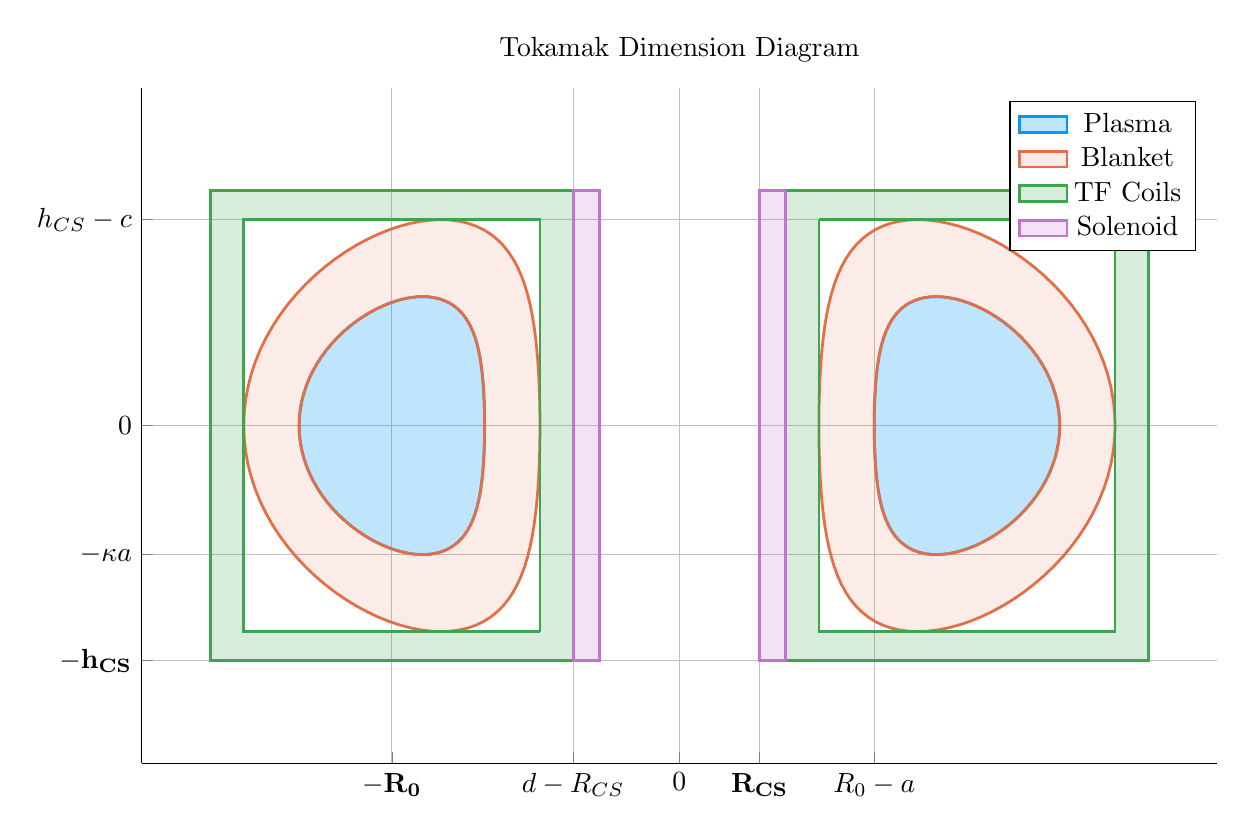
\begin{tikzpicture}[]
\begin{axis}[height = {101.6mm}, ylabel = {}, title = {Tokamak Dimension Diagram}, xmin = {-16.96464}, xmax = {16.96464}, ymax = {12.181706012903225}, xlabel = {}, unbounded coords=jump,scaled x ticks = false,xticklabel style={rotate = 0},xmajorgrids = true,xtick = {0.0,2.5317214541730677,-9.072,6.145548387096774,-3.3497214541730678},xticklabels = {0,$\bf{R_{CS}}$,$\bf{{-R}_0}$,$R_0 - a$,$d - R_{CS}$},xtick align = inside,axis lines* = left,scaled y ticks = false,yticklabel style={rotate = 0},ymajorgrids = true,ytick = {0.0,-8.478922887864822,-4.653058064516129,7.428922887864823},yticklabels = {0,$\bf{{-h}_{CS}}$,${-\kappa} a$,$h_{CS} - c$},ytick align = inside,axis lines* = left,    xshift = 0.0mm,
    yshift = 0.0mm,
    axis background/.style={fill={rgb,1:red,1.00000000;green,1.00000000;blue,1.00000000}}
, ymin = {-12.181706012903225}, width = {152.4mm}]\addplot+ [color = {rgb,1:red,0.00000000;green,0.60560316;blue,0.97868012},
draw opacity=1.0,
line width=1,
solid,mark = none,
mark size = 2.0,
mark options = {
    color = {rgb,1:red,0.00000000;green,0.00000000;blue,0.00000000}, draw opacity = 1.0,
    fill = {rgb,1:red,0.00000000;green,0.60560316;blue,0.97868012}, fill opacity = 1.0,
    line width = 1,
    rotate = 0,
    solid
},fill = {rgb,1:red,0.00000000;green,0.60560316;blue,0.97868012}, fill opacity=0.25,area legend]coordinates {
(-11.998451612903224, 0.0)
(-11.98922207919679, 0.2921679332710291)
(-11.961601612443932, 0.5831828131882695)
(-11.915794116436746, 0.8718961369727396)
(-11.852137762522407, 1.1571684850360338)
(-11.771102473770108, 1.4378740177488842)
(-11.673286377647635, 1.7129049186158334)
(-11.55941120568557, 1.9811757663208256)
(-11.430316617462449, 2.241627818389261)
(-11.286953428530017, 2.4932331895608506)
(-11.130375728034215, 2.7349989083831394)
(-10.96173188200961, 2.9659708360161865)
(-10.782254432669117, 3.1852374317826615)
(-10.59324892230544, 3.391933350602452)
(-10.396081692289423, 3.58524285811436)
(-10.192166732519574, 3.7644030500069485)
(-9.982951683794182, 3.9287068628533244)
(-9.769903124035281, 4.0775058645674545)
(-9.554491298062636, 4.21021281346937)
(-9.338174478579997, 4.326303975859794)
(-9.122383172034585, 4.425321192957779)
(-8.908504405883159, 4.5068736890441015)
(-8.697866352426912, 4.570639613674501)
(-8.491723557735288, 4.616367311876341)
(-8.2912430513685, 4.643876317315818)
(-8.097491612903225, 4.653058064516129)
(-7.911424464141755, 4.643876317315818)
(-7.73387564104738, 4.616367311876341)
(-7.565550276852846, 4.570639613674501)
(-7.4070189976483904, 4.506873689044102)
(-7.258714594546428, 4.42532119295778)
(-7.120931092970638, 4.326303975859795)
(-6.993825290693801, 4.21021281346937)
(-6.877420783129728, 4.077505864567455)
(-6.771614438426758, 3.928706862853325)
(-6.676185227609827, 3.7644030500069485)
(-6.590805257964794, 3.58524285811436)
(-6.515052802686304, 3.391933350602452)
(-6.448427068145589, 3.1852374317826624)
(-6.390364393542622, 2.9659708360161874)
(-6.340255537642832, 2.73499890838314)
(-6.297463675055492, 2.4932331895608506)
(-6.261342701178994, 2.241627818389261)
(-6.231255431364441, 1.9811757663208265)
(-6.206591276608178, 1.7129049186158343)
(-6.186782985455325, 1.4378740177488847)
(-6.171322059752492, 1.1571684850360338)
(-6.159772480089943, 0.8718961369727395)
(-6.151782414579849, 0.5831828131882707)
(-6.147093631099405, 0.29216793327103)
(-6.145548387096774, 5.698352664956456e-16)
(-6.147093631099405, -0.2921679332710289)
(-6.151782414579849, -0.5831828131882696)
(-6.159772480089943, -0.8718961369727383)
(-6.171322059752492, -1.1571684850360326)
(-6.1867829854553245, -1.4378740177488838)
(-6.206591276608178, -1.7129049186158334)
(-6.231255431364441, -1.9811757663208256)
(-6.261342701178992, -2.2416278183892597)
(-6.297463675055493, -2.4932331895608497)
(-6.340255537642832, -2.734998908383139)
(-6.390364393542622, -2.9659708360161865)
(-6.448427068145589, -3.185237431782662)
(-6.515052802686304, -3.3919333506024514)
(-6.590805257964794, -3.5852428581143605)
(-6.676185227609827, -3.7644030500069485)
(-6.771614438426755, -3.928706862853323)
(-6.877420783129727, -4.0775058645674545)
(-6.9938252906938, -4.21021281346937)
(-7.120931092970639, -4.326303975859795)
(-7.258714594546428, -4.425321192957779)
(-7.407018997648389, -4.5068736890441015)
(-7.565550276852846, -4.570639613674501)
(-7.733875641047377, -4.616367311876341)
(-7.9114244641417555, -4.643876317315818)
(-8.097491612903225, -4.653058064516129)
(-8.291243051368498, -4.643876317315818)
(-8.491723557735288, -4.616367311876341)
(-8.69786635242691, -4.570639613674501)
(-8.90850440588316, -4.5068736890441015)
(-9.122383172034585, -4.42532119295778)
(-9.338174478579994, -4.326303975859796)
(-9.554491298062636, -4.21021281346937)
(-9.76990312403528, -4.077505864567455)
(-9.982951683794184, -3.928706862853324)
(-10.192166732519574, -3.7644030500069494)
(-10.396081692289421, -3.5852428581143614)
(-10.59324892230544, -3.391933350602452)
(-10.782254432669115, -3.1852374317826624)
(-10.96173188200961, -2.9659708360161865)
(-11.130375728034215, -2.7349989083831403)
(-11.286953428530017, -2.493233189560853)
(-11.430316617462449, -2.241627818389261)
(-11.559411205685569, -1.981175766320827)
(-11.673286377647635, -1.7129049186158327)
(-11.771102473770108, -1.4378740177488853)
(-11.852137762522407, -1.1571684850360362)
(-11.915794116436746, -0.8718961369727398)
(-11.961601612443932, -0.5831828131882713)
(-11.98922207919679, -0.2921679332710286)
(-11.998451612903224, -1.1396705329912913e-15)
(NaN, NaN)
(11.998451612903224, 0.0)
(11.98922207919679, 0.2921679332710291)
(11.961601612443932, 0.5831828131882695)
(11.915794116436746, 0.8718961369727396)
(11.852137762522407, 1.1571684850360338)
(11.771102473770108, 1.4378740177488842)
(11.673286377647635, 1.7129049186158334)
(11.55941120568557, 1.9811757663208256)
(11.430316617462449, 2.241627818389261)
(11.286953428530017, 2.4932331895608506)
(11.130375728034215, 2.7349989083831394)
(10.96173188200961, 2.9659708360161865)
(10.782254432669117, 3.1852374317826615)
(10.59324892230544, 3.391933350602452)
(10.396081692289423, 3.58524285811436)
(10.192166732519574, 3.7644030500069485)
(9.982951683794182, 3.9287068628533244)
(9.769903124035281, 4.0775058645674545)
(9.554491298062636, 4.21021281346937)
(9.338174478579997, 4.326303975859794)
(9.122383172034585, 4.425321192957779)
(8.908504405883159, 4.5068736890441015)
(8.697866352426912, 4.570639613674501)
(8.491723557735288, 4.616367311876341)
(8.2912430513685, 4.643876317315818)
(8.097491612903225, 4.653058064516129)
(7.911424464141755, 4.643876317315818)
(7.73387564104738, 4.616367311876341)
(7.565550276852846, 4.570639613674501)
(7.4070189976483904, 4.506873689044102)
(7.258714594546428, 4.42532119295778)
(7.120931092970638, 4.326303975859795)
(6.993825290693801, 4.21021281346937)
(6.877420783129728, 4.077505864567455)
(6.771614438426758, 3.928706862853325)
(6.676185227609827, 3.7644030500069485)
(6.590805257964794, 3.58524285811436)
(6.515052802686304, 3.391933350602452)
(6.448427068145589, 3.1852374317826624)
(6.390364393542622, 2.9659708360161874)
(6.340255537642832, 2.73499890838314)
(6.297463675055492, 2.4932331895608506)
(6.261342701178994, 2.241627818389261)
(6.231255431364441, 1.9811757663208265)
(6.206591276608178, 1.7129049186158343)
(6.186782985455325, 1.4378740177488847)
(6.171322059752492, 1.1571684850360338)
(6.159772480089943, 0.8718961369727395)
(6.151782414579849, 0.5831828131882707)
(6.147093631099405, 0.29216793327103)
(6.145548387096774, 5.698352664956456e-16)
(6.147093631099405, -0.2921679332710289)
(6.151782414579849, -0.5831828131882696)
(6.159772480089943, -0.8718961369727383)
(6.171322059752492, -1.1571684850360326)
(6.1867829854553245, -1.4378740177488838)
(6.206591276608178, -1.7129049186158334)
(6.231255431364441, -1.9811757663208256)
(6.261342701178992, -2.2416278183892597)
(6.297463675055493, -2.4932331895608497)
(6.340255537642832, -2.734998908383139)
(6.390364393542622, -2.9659708360161865)
(6.448427068145589, -3.185237431782662)
(6.515052802686304, -3.3919333506024514)
(6.590805257964794, -3.5852428581143605)
(6.676185227609827, -3.7644030500069485)
(6.771614438426755, -3.928706862853323)
(6.877420783129727, -4.0775058645674545)
(6.9938252906938, -4.21021281346937)
(7.120931092970639, -4.326303975859795)
(7.258714594546428, -4.425321192957779)
(7.407018997648389, -4.5068736890441015)
(7.565550276852846, -4.570639613674501)
(7.733875641047377, -4.616367311876341)
(7.9114244641417555, -4.643876317315818)
(8.097491612903225, -4.653058064516129)
(8.291243051368498, -4.643876317315818)
(8.491723557735288, -4.616367311876341)
(8.69786635242691, -4.570639613674501)
(8.90850440588316, -4.5068736890441015)
(9.122383172034585, -4.42532119295778)
(9.338174478579994, -4.326303975859796)
(9.554491298062636, -4.21021281346937)
(9.76990312403528, -4.077505864567455)
(9.982951683794184, -3.928706862853324)
(10.192166732519574, -3.7644030500069494)
(10.396081692289421, -3.5852428581143614)
(10.59324892230544, -3.391933350602452)
(10.782254432669115, -3.1852374317826624)
(10.96173188200961, -2.9659708360161865)
(11.130375728034215, -2.7349989083831403)
(11.286953428530017, -2.493233189560853)
(11.430316617462449, -2.241627818389261)
(11.559411205685569, -1.981175766320827)
(11.673286377647635, -1.7129049186158327)
(11.771102473770108, -1.4378740177488853)
(11.852137762522407, -1.1571684850360362)
(11.915794116436746, -0.8718961369727398)
(11.961601612443932, -0.5831828131882713)
(11.98922207919679, -0.2921679332710286)
(11.998451612903224, -1.1396705329912913e-15)
};
\addlegendentry{Plasma}
\addplot+ [color = {rgb,1:red,0.88887350;green,0.43564919;blue,0.27812294},
draw opacity=1.0,
line width=1,
solid,mark = none,
mark size = 2.0,
mark options = {
    color = {rgb,1:red,0.00000000;green,0.00000000;blue,0.00000000}, draw opacity = 1.0,
    fill = {rgb,1:red,0.88887350;green,0.43564919;blue,0.27812294}, fill opacity = 1.0,
    line width = 1,
    rotate = 0,
    solid
},fill = {rgb,1:red,0.88887350;green,0.43564919;blue,0.27812294}, fill opacity=0.125,area legend]coordinates {
(-13.74427854582693, 0.0)
(-13.72954296908463, 0.46646592767223927)
(-13.685445019996358, 0.9310909274359673)
(-13.612310244800092, 1.392041336684088)
(-13.510678556994915, 1.8474979947395098)
(-13.381300220642846, 2.2956634222512418)
(-13.225130186826302, 2.734768915024204)
(-13.04332074889991, 3.1630815242866377)
(-12.837212480347718, 3.5789108958472036)
(-12.608323422706404, 3.9806159411507194)
(-12.358336500812388, 4.3666113139049525)
(-12.08908515895104, 4.735373666718153)
(-11.802537234387401, 5.08544766305526)
(-11.500777113966619, 5.4154517207863275)
(-11.185986254387002, 5.724083464660006)
(-10.860422186454013, 6.010124866183653)
(-10.526396166917667, 6.272447050625345)
(-10.18624968693083, 6.510014752166694)
(-9.842330092097374, 6.721890399624077)
(-9.496965613725703, 6.907237816613755)
(-9.152440152411872, 7.065325521558049)
(-8.81096819159381, 7.195529614508949)
(-8.474670248460548, 7.297336239396166)
(-8.14554929092694, 7.370343611982296)
(-7.825468560863273, 7.4142636055216355)
(-7.516131244239631, 7.428922887864823)
(-7.2190624174706315, 7.4142636055216355)
(-6.935593675557043, 7.370343611982296)
(-6.666850811544881, 7.297336239396167)
(-6.4137448687014755, 7.195529614508949)
(-6.176966827400615, 7.065325521558051)
(-5.956986119179431, 6.907237816613756)
(-5.754053082320152, 6.721890399624076)
(-5.568205388501765, 6.510014752166695)
(-5.3992783807260825, 6.272447050625345)
(-5.246919171238659, 6.010124866183653)
(-5.110604257075394, 5.724083464660006)
(-4.989660322779391, 5.4154517207863275)
(-4.88328781734585, 5.085447663055262)
(-4.790586818065825, 4.735373666718154)
(-4.7105846299742, 4.366611313904953)
(-4.642264518129107, 3.9806159411507194)
(-4.584594932698949, 3.578910895847203)
(-4.536558565161822, 3.1630815242866395)
(-4.497180568747824, 2.7347689150242047)
(-4.465555288023927, 2.2956634222512426)
(-4.440870871189059, 1.8474979947395103)
(-4.422431183673739, 1.3920413366840876)
(-4.409674501998921, 0.9310909274359696)
(-4.402188541060726, 0.46646592767224077)
(-4.399721454173068, 9.097806635736167e-16)
(-4.402188541060726, -0.466465927672239)
(-4.409674501998921, -0.9310909274359678)
(-4.422431183673739, -1.392041336684086)
(-4.440870871189059, -1.8474979947395083)
(-4.465555288023926, -2.295663422251241)
(-4.497180568747823, -2.734768915024204)
(-4.536558565161822, -3.1630815242866377)
(-4.5845949326989475, -3.5789108958472013)
(-4.642264518129108, -3.980615941150719)
(-4.7105846299742, -4.3666113139049525)
(-4.790586818065825, -4.735373666718153)
(-4.88328781734585, -5.085447663055261)
(-4.989660322779391, -5.415451720786327)
(-5.110604257075395, -5.724083464660007)
(-5.246919171238659, -6.010124866183653)
(-5.399278380726081, -6.272447050625343)
(-5.568205388501764, -6.510014752166694)
(-5.754053082320152, -6.721890399624076)
(-5.956986119179432, -6.907237816613756)
(-6.176966827400615, -7.065325521558049)
(-6.413744868701472, -7.195529614508947)
(-6.666850811544881, -7.297336239396167)
(-6.935593675557041, -7.370343611982296)
(-7.219062417470632, -7.4142636055216355)
(-7.51613124423963, -7.428922887864823)
(-7.8254685608632695, -7.4142636055216355)
(-8.14554929092694, -7.370343611982296)
(-8.474670248460544, -7.297336239396167)
(-8.810968191593812, -7.195529614508949)
(-9.152440152411872, -7.065325521558051)
(-9.4969656137257, -6.9072378166137565)
(-9.842330092097372, -6.721890399624077)
(-10.186249686930825, -6.510014752166696)
(-10.526396166917669, -6.272447050625344)
(-10.860422186454013, -6.010124866183654)
(-11.185986254386998, -5.724083464660007)
(-11.500777113966619, -5.4154517207863275)
(-11.8025372343874, -5.085447663055262)
(-12.08908515895104, -4.735373666718153)
(-12.358336500812388, -4.366611313904954)
(-12.608323422706402, -3.9806159411507234)
(-12.837212480347718, -3.5789108958472036)
(-13.04332074889991, -3.1630815242866404)
(-13.225130186826302, -2.7347689150242034)
(-13.381300220642846, -2.2956634222512435)
(-13.510678556994915, -1.8474979947395136)
(-13.612310244800092, -1.3920413366840885)
(-13.685445019996358, -0.9310909274359703)
(-13.72954296908463, -0.46646592767223843)
(-13.74427854582693, -1.8195613271472333e-15)
(NaN, NaN)
(13.74427854582693, 0.0)
(13.72954296908463, 0.46646592767223927)
(13.685445019996358, 0.9310909274359673)
(13.612310244800092, 1.392041336684088)
(13.510678556994915, 1.8474979947395098)
(13.381300220642846, 2.2956634222512418)
(13.225130186826302, 2.734768915024204)
(13.04332074889991, 3.1630815242866377)
(12.837212480347718, 3.5789108958472036)
(12.608323422706404, 3.9806159411507194)
(12.358336500812388, 4.3666113139049525)
(12.08908515895104, 4.735373666718153)
(11.802537234387401, 5.08544766305526)
(11.500777113966619, 5.4154517207863275)
(11.185986254387002, 5.724083464660006)
(10.860422186454013, 6.010124866183653)
(10.526396166917667, 6.272447050625345)
(10.18624968693083, 6.510014752166694)
(9.842330092097374, 6.721890399624077)
(9.496965613725703, 6.907237816613755)
(9.152440152411872, 7.065325521558049)
(8.81096819159381, 7.195529614508949)
(8.474670248460548, 7.297336239396166)
(8.14554929092694, 7.370343611982296)
(7.825468560863273, 7.4142636055216355)
(7.516131244239631, 7.428922887864823)
(7.2190624174706315, 7.4142636055216355)
(6.935593675557043, 7.370343611982296)
(6.666850811544881, 7.297336239396167)
(6.4137448687014755, 7.195529614508949)
(6.176966827400615, 7.065325521558051)
(5.956986119179431, 6.907237816613756)
(5.754053082320152, 6.721890399624076)
(5.568205388501765, 6.510014752166695)
(5.3992783807260825, 6.272447050625345)
(5.246919171238659, 6.010124866183653)
(5.110604257075394, 5.724083464660006)
(4.989660322779391, 5.4154517207863275)
(4.88328781734585, 5.085447663055262)
(4.790586818065825, 4.735373666718154)
(4.7105846299742, 4.366611313904953)
(4.642264518129107, 3.9806159411507194)
(4.584594932698949, 3.578910895847203)
(4.536558565161822, 3.1630815242866395)
(4.497180568747824, 2.7347689150242047)
(4.465555288023927, 2.2956634222512426)
(4.440870871189059, 1.8474979947395103)
(4.422431183673739, 1.3920413366840876)
(4.409674501998921, 0.9310909274359696)
(4.402188541060726, 0.46646592767224077)
(4.399721454173068, 9.097806635736167e-16)
(4.402188541060726, -0.466465927672239)
(4.409674501998921, -0.9310909274359678)
(4.422431183673739, -1.392041336684086)
(4.440870871189059, -1.8474979947395083)
(4.465555288023926, -2.295663422251241)
(4.497180568747823, -2.734768915024204)
(4.536558565161822, -3.1630815242866377)
(4.5845949326989475, -3.5789108958472013)
(4.642264518129108, -3.980615941150719)
(4.7105846299742, -4.3666113139049525)
(4.790586818065825, -4.735373666718153)
(4.88328781734585, -5.085447663055261)
(4.989660322779391, -5.415451720786327)
(5.110604257075395, -5.724083464660007)
(5.246919171238659, -6.010124866183653)
(5.399278380726081, -6.272447050625343)
(5.568205388501764, -6.510014752166694)
(5.754053082320152, -6.721890399624076)
(5.956986119179432, -6.907237816613756)
(6.176966827400615, -7.065325521558049)
(6.413744868701472, -7.195529614508947)
(6.666850811544881, -7.297336239396167)
(6.935593675557041, -7.370343611982296)
(7.219062417470632, -7.4142636055216355)
(7.51613124423963, -7.428922887864823)
(7.8254685608632695, -7.4142636055216355)
(8.14554929092694, -7.370343611982296)
(8.474670248460544, -7.297336239396167)
(8.810968191593812, -7.195529614508949)
(9.152440152411872, -7.065325521558051)
(9.4969656137257, -6.9072378166137565)
(9.842330092097372, -6.721890399624077)
(10.186249686930825, -6.510014752166696)
(10.526396166917669, -6.272447050625344)
(10.860422186454013, -6.010124866183654)
(11.185986254386998, -5.724083464660007)
(11.500777113966619, -5.4154517207863275)
(11.8025372343874, -5.085447663055262)
(12.08908515895104, -4.735373666718153)
(12.358336500812388, -4.366611313904954)
(12.608323422706402, -3.9806159411507234)
(12.837212480347718, -3.5789108958472036)
(13.04332074889991, -3.1630815242866404)
(13.225130186826302, -2.7347689150242034)
(13.381300220642846, -2.2956634222512435)
(13.510678556994915, -1.8474979947395136)
(13.612310244800092, -1.3920413366840885)
(13.685445019996358, -0.9310909274359703)
(13.72954296908463, -0.46646592767223843)
(13.74427854582693, -1.8195613271472333e-15)
(NaN, NaN)
(11.998451612903224, -1.1396705329912913e-15)
(11.98922207919679, -0.2921679332710286)
(11.961601612443932, -0.5831828131882713)
(11.915794116436746, -0.8718961369727398)
(11.852137762522407, -1.1571684850360362)
(11.771102473770108, -1.4378740177488853)
(11.673286377647635, -1.7129049186158327)
(11.55941120568557, -1.981175766320827)
(11.430316617462449, -2.241627818389261)
(11.286953428530017, -2.493233189560853)
(11.130375728034215, -2.7349989083831403)
(10.96173188200961, -2.9659708360161865)
(10.782254432669117, -3.1852374317826624)
(10.59324892230544, -3.391933350602452)
(10.396081692289423, -3.5852428581143614)
(10.192166732519574, -3.7644030500069494)
(9.982951683794182, -3.928706862853324)
(9.769903124035281, -4.077505864567455)
(9.554491298062636, -4.21021281346937)
(9.338174478579997, -4.326303975859796)
(9.122383172034585, -4.42532119295778)
(8.908504405883159, -4.5068736890441015)
(8.697866352426912, -4.570639613674501)
(8.491723557735288, -4.616367311876341)
(8.2912430513685, -4.643876317315818)
(8.097491612903225, -4.653058064516129)
(7.911424464141755, -4.643876317315818)
(7.73387564104738, -4.616367311876341)
(7.565550276852846, -4.570639613674501)
(7.4070189976483904, -4.5068736890441015)
(7.258714594546428, -4.425321192957779)
(7.120931092970638, -4.326303975859795)
(6.993825290693801, -4.21021281346937)
(6.877420783129728, -4.0775058645674545)
(6.771614438426758, -3.928706862853323)
(6.676185227609827, -3.7644030500069485)
(6.590805257964794, -3.5852428581143605)
(6.515052802686304, -3.3919333506024514)
(6.448427068145589, -3.185237431782662)
(6.390364393542622, -2.9659708360161865)
(6.340255537642832, -2.734998908383139)
(6.297463675055492, -2.4932331895608497)
(6.261342701178994, -2.2416278183892597)
(6.231255431364441, -1.9811757663208256)
(6.206591276608178, -1.7129049186158334)
(6.186782985455325, -1.4378740177488838)
(6.171322059752492, -1.1571684850360326)
(6.159772480089943, -0.8718961369727383)
(6.151782414579849, -0.5831828131882696)
(6.147093631099405, -0.2921679332710289)
(6.145548387096774, 5.698352664956456e-16)
(6.147093631099405, 0.29216793327103)
(6.151782414579849, 0.5831828131882707)
(6.159772480089943, 0.8718961369727395)
(6.171322059752492, 1.1571684850360338)
(6.1867829854553245, 1.4378740177488847)
(6.206591276608178, 1.7129049186158343)
(6.231255431364441, 1.9811757663208265)
(6.261342701178992, 2.241627818389261)
(6.297463675055493, 2.4932331895608506)
(6.340255537642832, 2.73499890838314)
(6.390364393542622, 2.9659708360161874)
(6.448427068145589, 3.1852374317826624)
(6.515052802686304, 3.391933350602452)
(6.590805257964794, 3.58524285811436)
(6.676185227609827, 3.7644030500069485)
(6.771614438426755, 3.928706862853325)
(6.877420783129727, 4.077505864567455)
(6.9938252906938, 4.21021281346937)
(7.120931092970639, 4.326303975859795)
(7.258714594546428, 4.42532119295778)
(7.407018997648389, 4.506873689044102)
(7.565550276852846, 4.570639613674501)
(7.733875641047377, 4.616367311876341)
(7.9114244641417555, 4.643876317315818)
(8.097491612903225, 4.653058064516129)
(8.291243051368498, 4.643876317315818)
(8.491723557735288, 4.616367311876341)
(8.69786635242691, 4.570639613674501)
(8.90850440588316, 4.5068736890441015)
(9.122383172034585, 4.425321192957779)
(9.338174478579994, 4.326303975859794)
(9.554491298062636, 4.21021281346937)
(9.76990312403528, 4.0775058645674545)
(9.982951683794184, 3.9287068628533244)
(10.192166732519574, 3.7644030500069485)
(10.396081692289421, 3.58524285811436)
(10.59324892230544, 3.391933350602452)
(10.782254432669115, 3.1852374317826615)
(10.96173188200961, 2.9659708360161865)
(11.130375728034215, 2.7349989083831394)
(11.286953428530017, 2.4932331895608506)
(11.430316617462449, 2.241627818389261)
(11.559411205685569, 1.9811757663208256)
(11.673286377647635, 1.7129049186158334)
(11.771102473770108, 1.4378740177488842)
(11.852137762522407, 1.1571684850360338)
(11.915794116436746, 0.8718961369727396)
(11.961601612443932, 0.5831828131882695)
(11.98922207919679, 0.2921679332710291)
(11.998451612903224, 0.0)
(NaN, NaN)
(-11.998451612903224, -1.1396705329912913e-15)
(-11.98922207919679, -0.2921679332710286)
(-11.961601612443932, -0.5831828131882713)
(-11.915794116436746, -0.8718961369727398)
(-11.852137762522407, -1.1571684850360362)
(-11.771102473770108, -1.4378740177488853)
(-11.673286377647635, -1.7129049186158327)
(-11.55941120568557, -1.981175766320827)
(-11.430316617462449, -2.241627818389261)
(-11.286953428530017, -2.493233189560853)
(-11.130375728034215, -2.7349989083831403)
(-10.96173188200961, -2.9659708360161865)
(-10.782254432669117, -3.1852374317826624)
(-10.59324892230544, -3.391933350602452)
(-10.396081692289423, -3.5852428581143614)
(-10.192166732519574, -3.7644030500069494)
(-9.982951683794182, -3.928706862853324)
(-9.769903124035281, -4.077505864567455)
(-9.554491298062636, -4.21021281346937)
(-9.338174478579997, -4.326303975859796)
(-9.122383172034585, -4.42532119295778)
(-8.908504405883159, -4.5068736890441015)
(-8.697866352426912, -4.570639613674501)
(-8.491723557735288, -4.616367311876341)
(-8.2912430513685, -4.643876317315818)
(-8.097491612903225, -4.653058064516129)
(-7.911424464141755, -4.643876317315818)
(-7.73387564104738, -4.616367311876341)
(-7.565550276852846, -4.570639613674501)
(-7.4070189976483904, -4.5068736890441015)
(-7.258714594546428, -4.425321192957779)
(-7.120931092970638, -4.326303975859795)
(-6.993825290693801, -4.21021281346937)
(-6.877420783129728, -4.0775058645674545)
(-6.771614438426758, -3.928706862853323)
(-6.676185227609827, -3.7644030500069485)
(-6.590805257964794, -3.5852428581143605)
(-6.515052802686304, -3.3919333506024514)
(-6.448427068145589, -3.185237431782662)
(-6.390364393542622, -2.9659708360161865)
(-6.340255537642832, -2.734998908383139)
(-6.297463675055492, -2.4932331895608497)
(-6.261342701178994, -2.2416278183892597)
(-6.231255431364441, -1.9811757663208256)
(-6.206591276608178, -1.7129049186158334)
(-6.186782985455325, -1.4378740177488838)
(-6.171322059752492, -1.1571684850360326)
(-6.159772480089943, -0.8718961369727383)
(-6.151782414579849, -0.5831828131882696)
(-6.147093631099405, -0.2921679332710289)
(-6.145548387096774, 5.698352664956456e-16)
(-6.147093631099405, 0.29216793327103)
(-6.151782414579849, 0.5831828131882707)
(-6.159772480089943, 0.8718961369727395)
(-6.171322059752492, 1.1571684850360338)
(-6.1867829854553245, 1.4378740177488847)
(-6.206591276608178, 1.7129049186158343)
(-6.231255431364441, 1.9811757663208265)
(-6.261342701178992, 2.241627818389261)
(-6.297463675055493, 2.4932331895608506)
(-6.340255537642832, 2.73499890838314)
(-6.390364393542622, 2.9659708360161874)
(-6.448427068145589, 3.1852374317826624)
(-6.515052802686304, 3.391933350602452)
(-6.590805257964794, 3.58524285811436)
(-6.676185227609827, 3.7644030500069485)
(-6.771614438426755, 3.928706862853325)
(-6.877420783129727, 4.077505864567455)
(-6.9938252906938, 4.21021281346937)
(-7.120931092970639, 4.326303975859795)
(-7.258714594546428, 4.42532119295778)
(-7.407018997648389, 4.506873689044102)
(-7.565550276852846, 4.570639613674501)
(-7.733875641047377, 4.616367311876341)
(-7.9114244641417555, 4.643876317315818)
(-8.097491612903225, 4.653058064516129)
(-8.291243051368498, 4.643876317315818)
(-8.491723557735288, 4.616367311876341)
(-8.69786635242691, 4.570639613674501)
(-8.90850440588316, 4.5068736890441015)
(-9.122383172034585, 4.425321192957779)
(-9.338174478579994, 4.326303975859794)
(-9.554491298062636, 4.21021281346937)
(-9.76990312403528, 4.0775058645674545)
(-9.982951683794184, 3.9287068628533244)
(-10.192166732519574, 3.7644030500069485)
(-10.396081692289421, 3.58524285811436)
(-10.59324892230544, 3.391933350602452)
(-10.782254432669115, 3.1852374317826615)
(-10.96173188200961, 2.9659708360161865)
(-11.130375728034215, 2.7349989083831394)
(-11.286953428530017, 2.4932331895608506)
(-11.430316617462449, 2.241627818389261)
(-11.559411205685569, 1.9811757663208256)
(-11.673286377647635, 1.7129049186158334)
(-11.771102473770108, 1.4378740177488842)
(-11.852137762522407, 1.1571684850360338)
(-11.915794116436746, 0.8718961369727396)
(-11.961601612443932, 0.5831828131882695)
(-11.98922207919679, 0.2921679332710291)
(-11.998451612903224, 0.0)
};
\addlegendentry{Blanket}
\addplot+ [color = {rgb,1:red,0.24222430;green,0.64327509;blue,0.30444865},
draw opacity=1.0,
line width=1,
solid,mark = none,
mark size = 2.0,
mark options = {
    color = {rgb,1:red,0.00000000;green,0.00000000;blue,0.00000000}, draw opacity = 1.0,
    fill = {rgb,1:red,0.24222430;green,0.64327509;blue,0.30444865}, fill opacity = 1.0,
    line width = 1,
    rotate = 0,
    solid
},fill = {rgb,1:red,0.24222430;green,0.64327509;blue,0.30444865}, fill opacity=0.2,area legend]coordinates {
(-4.399721454173068, -7.428922887864823)
(-13.74427854582693, -7.428922887864823)
(-13.74427854582693, 7.428922887864823)
(-4.399721454173068, 7.428922887864823)
(-4.399721454173068, -7.428922887864823)
(NaN, NaN)
(-3.3497214541730678, -8.478922887864822)
(-3.3497214541730678, 8.478922887864822)
(-14.79427854582693, 8.478922887864822)
(-14.79427854582693, -8.478922887864822)
(-3.3497214541730678, -8.478922887864822)
(NaN, NaN)
(4.399721454173068, 7.428922887864823)
(13.74427854582693, 7.428922887864823)
(13.74427854582693, -7.428922887864823)
(4.399721454173068, -7.428922887864823)
(4.399721454173068, 7.428922887864823)
(NaN, NaN)
(3.3497214541730678, 8.478922887864822)
(3.3497214541730678, -8.478922887864822)
(14.79427854582693, -8.478922887864822)
(14.79427854582693, 8.478922887864822)
(3.3497214541730678, 8.478922887864822)
};
\addlegendentry{TF Coils}
\addplot+ [color = {rgb,1:red,0.76444018;green,0.44411178;blue,0.82429754},
draw opacity=1.0,
line width=1,
solid,mark = none,
mark size = 2.0,
mark options = {
    color = {rgb,1:red,0.00000000;green,0.00000000;blue,0.00000000}, draw opacity = 1.0,
    fill = {rgb,1:red,0.76444018;green,0.44411178;blue,0.82429754}, fill opacity = 1.0,
    line width = 1,
    rotate = 0,
    solid
},fill = {rgb,1:red,0.76444018;green,0.44411178;blue,0.82429754}, fill opacity=0.2,area legend]coordinates {
(-3.3497214541730678, -8.478922887864822)
(-3.3497214541730678, 8.478922887864822)
(-2.5317214541730677, 8.478922887864822)
(-2.5317214541730677, -8.478922887864822)
(-3.3497214541730678, -8.478922887864822)
(NaN, NaN)
(3.3497214541730678, 8.478922887864822)
(3.3497214541730678, -8.478922887864822)
(2.5317214541730677, -8.478922887864822)
(2.5317214541730677, 8.478922887864822)
(3.3497214541730678, 8.478922887864822)
};
\addlegendentry{Solenoid}
\end{axis}

\end{tikzpicture}

\end{adjustbox}

\caption{Dimensions of Tokamak Cross-Section}
\label{fig:dims} ~ \\
\small{Geometrically, a tokamak consists mainly of four components: the plasma, it's metallic blanket, the toroidal field magnets surrounding them, and the central solenoid. These have thicknesses of a, b, c and d, respectively. $R_{CS}$ is where the solenoid starts.}
\end{figure*}

The blanket and TF coils have thicknesses of $b$ and $c$, respectively. Before defining $b$, $c$, and $d$, though, it proves fruitful to relate all the quantities in equations for the inner radius ($R_{CS}$) and height ($h_{CS}$) of the central solenoid.
 \begin{gather}
 	\label{eq:rcs1}
 	R_{CS} = R_0 - ( a + b + c + d ) \\
	\label{eq:hcs1}
 	h_{CS} = 2 \cdot \left ( \kappa a + b + c \right)
 \end{gather}
Again, this relation is pictorially represented in \cref{fig:dims}. The next step is defining: $b$, $c$, and $d$ -- to close the variable loop.

\subsection{\replaced{Calculating}{Measuring} Component Thicknesses}

In between the inner surface of the central solenoid and the major radius of the tokamak are four thicknesses: $a$, $b$, $c$, and $d$. This subsection will go over them one-by-one.

\subsubsection{The Minor Radius -- $a$}

The minor radius was the first of these thicknesses we encountered. To calculate it, we introduced the inverse aspect ratio ($\varepsilon$) to relate it to the major radius ($R_0$):
\begin{equation}
	\tag{\ref{eq:a}}
	a = \varepsilon \cdot R_0
\end{equation}

\subsubsection{The Blanket Thickness -- $b$}

The blanket is an area between the TF coils and the torus that is \deleted{strongly}composed \added{mainly} of lithium \added{and steel}. It serves to both: protect the superconducting magnet structures from neutron damage, as well as breed \deleted{a little}more tritium fuel from stray fusion neutrons.\cite{blanket} In equation form, the blanket thickness is given by: \cite{minervini}
\begin{equation}
	\label{eq:bb}
	\tcboxmath{
	b = 1.23 + 0.074 \ \textnormal{ln} \, P_W
	}
\end{equation}
\myequations{Blanket Thickness -- $b$}
\replaced{Here, $P_W$}{Here, the constant term (i.e.\ 1.23) is approximately the mean-free-path of fusion neutrons through lithium-7 -- the thickness of lithium needed to reduce the population of neutrons by $\sim 65\%$. While the second term, which includes $P_W$,} is a correction to account for extra wall loading (as discussed in \replaced{\cref{subsection:wall_loading}}{the secondary constraint section}).

Moving forward, the remaining two thicknesses -- $c$ and $d$ -- are handled differently, estimating structural steel portions as well as magnetic current-carrying ones.

\subsubsection{The Toroidal Field Coil Thickness -- $c$}

The thickness of the TF coils -- $c$ -- is a little beyond the scope of this paper. It does, however, have a form that combines a structural steel component with a magnetic portion. From \replaced{a previous model}{one of Jeff's previous models}, this can be given as: \cite{minervini}
\begin{equation}
	\label{eq:cc}
	\tcboxmath{
	c = G_{CI} R_0 + G_{CO}
	}
\end{equation}
\myequations{TF Coil Thickness -- $c$}
\begin{gather}
	G_{CI} = \frac{B_{0}^2}{ 4 \mu_0 \sigma_{TF} } \cdot \frac{1}{ ( 1 - \varepsilon_b )}  \cdot \left( \frac{ 4 \, \varepsilon_b}{1+\varepsilon_b} + \ \textnormal{ln} \left( \frac{1+\varepsilon_b}{1-\varepsilon_b} \right) \right) \\
	G_{CO} = \frac{B_{0}}{ \mu_0 J_{TF} } \cdot \frac{1}{ ( 1 - \varepsilon_b )}
\end{gather}
The critical stress -- $\sigma_{TF}$ in $G_{CI}$ implies it depends on the structural component, whereas the maximum current density -- $J_{TF}$ -- implies a magnetic predisposition in $G_{CO}$. The use of $G_\square$ in these quantities, instead of $K_\square$ is because they include the toroidal magnetic field strength -- $B_0$. For this reason, they are referred to as \replaced{dynamic}{floating} coefficients. Lastly, the term $\varepsilon_b$ represents the blanket inverse aspect ratio that combines the minor radius with the blanket thickness:
\begin{equation}
	\varepsilon_b = \frac{ a + b }{R_0}
\end{equation}

\subsubsection{The Central Solenoid Thickness -- $d$}

Finishing this discussion where we started, the central solenoid's thickness -- $d$ -- has a form similar to the TF coil's (i.e.\ $c$). In mathematical form, this can be represented as: \cite{minervini}
 \begin{equation}
 	\label{eq:dd}
 	\tcboxmath{
	d = K_{DR} R_{CS} + K_{DO}
	}
\end{equation}
\myequations{Central Solenoid Thickness -- $d$}
\begin{equation}
	K_{DR} = \frac{3 B_{CS}^2}{ 6 \mu_0 \sigma_{CS}  - B_{CS}^2 }
\end{equation}
\begin{equation}
	K_{DO} = \frac{6 B_{CS} \sigma_{CS}}{ 6 \mu_0 \sigma_{CS}  - B_{CS}^2 } \cdot \left( \frac{1}{J_{OH}} \right)
\end{equation}

Here, the use of $K_\square$ for the coefficients signifies their use as \replaced{static}{fixed} coefficients. Therefore, $B_{CS}$ must be treated as a \replaced{static}{fixed} variable representing the magnetic field strength in the central solenoid. For prospective solenoids using high temperature superconducting (HTS) tape, $B_{CS}$ may be around 20\,T. The values of $\sigma_{CS}$ and $J_{CS}$ have similar meanings to the ones for TF coils. These are collected in a table below with example values representative of our model.

\begin{table}[h!]
\centering
\caption{Example TF Coils and Central Solenoid Critical Values}
\hfill
\begin{subtable}[t]{0.45\textwidth}
\centering
\caption{Stresses [MPa]} ~\\
\begin{tabular}{ c|c|c }

\textbf{Item} & \textbf{Symbol} & \textbf{Limit} \\
\hline
Solenoid & $\sigma_{CS}$ & \replaced{600}{300} \\
TF Coils & $\sigma_{TF}$ & 600 \\
\end{tabular}
\end{subtable}
\hfill
\begin{subtable}[t]{0.45\textwidth}
\centering
\caption{Current Densities [$\sfrac{\textnormal{MA}}{\textnormal{m}^2}$]} ~\\
\begin{tabular}{ c|c|c }

\textbf{Item} & \textbf{Symbol} & \textbf{Limit} \\
\hline
Solenoid & $J_{CS}$ & \replaced{100}{50} \\
TF Coils & $J_{TF}$ & 200 \\
\end{tabular}
\end{subtable}
\hfill
\hfill
\end{table}

Before moving on, it seems important to say that although $K_{DI}$ and $K_{DO}$ do not depend on \replaced{dynamic}{floating} variables, $R_{CS}$ most definitely does. This is what makes the central solenoid's thickness difficult.

\subsection{Revisiting Central Solenoid Dimensions}

Now that the various thicknesses have been defined (i.e.\ $a$, $b$, $c$, and $d$), the equations for the solenoid's dimensions (i.e.\ $R_{CS}$ and $h_{CS}$), can now be revisited and simplified. From before,
 \begin{gather}
 	\tag{\ref{eq:rcs1}}
 	R_{CS} = R_0 - ( a + b + c + d ) \\
	\tag{\ref{eq:hcs1}}
 	h_{CS} = 2 \cdot \left ( \kappa a + b + c \right)
 \end{gather}
Utilizing the four thicknesses from before, these can now be expanded to simple formulas. Repeating the thicknesses:
\begin{align}
	\tag{\ref{eq:a}}
	a &= \varepsilon \cdot R_0 \\
	\tag{\ref{eq:bb}}
	b &= 1.23 + 0.074 \ \textnormal{ln} \, P_W \\
	\tag{\ref{eq:cc}}
	c &= G_{CI} R_0 + G_{CO} \\
 	\tag{\ref{eq:dd}}
	d &= K_{DR} R_{CS} + K_{DO}
\end{align}
Plugging these into the central solenoid's dimensions results in:
\begin{equation}
	\tcbhighmath{
	h_{CS} = 2 \cdot \left( R_0 \cdot \left( \varepsilon \kappa + G_{CI} \right) + \left( b + G_{CO} \right) \right)
	}
\end{equation}
\myequations{Central Solenoid Height -- $h_{CS}$}
\begin{equation}
	\tcbhighmath{
	R_{CS} = \frac{ 1 }{ 1 + K_{DR} } \cdot \left( R_0 \cdot \left( 1 - \varepsilon - G_{CI}  \right) - \left( K_{DO} + b + G_{CO}  \right) \right)
	}
\end{equation}
\myequations{Central Solenoid Inner Radius -- $R_{CS}$}

These are the complete central solenoid dimension formulas. To make them more tractable to the reader, they will now be simplified one step at a time. (The same simplification exercise will be done again after the generalized current is derived later this chapter.)

The first simplification to make while estimating central solenoid dimensions is to neglect the magnetic current-carrying portions of the central solenoid and TF coils. This results in:
\begin{equation}
	\underset{K_{DO} \to 0}{\underset{G_{CO} \to 0}{\lim}} \ h_{CS} = h_{CS}^{\,\dagger} = 2 R_0 \cdot \left( K_{EK} + \varepsilon_b + G_{CI} \right)
\end{equation}
\begin{equation}
	\underset{K_{DO} \to 0}{\underset{G_{CO} \to 0}{\lim}} \ R_{CS} = R_{CS}^{\,\dagger} = \frac{ R_0 }{ 1 + K_{DR} } \cdot \left( 1 - \varepsilon_b - G_{CI}  \right)
\end{equation}

The new \replaced{static}{fixed} coefficient, here, is:
\begin{equation}
	K_{EK} = \varepsilon \cdot \left( \kappa - 1 \right)
\end{equation}
The next simplification is ignoring the TF coil thickness -- and thus magnetic field dependence -- altogether:
\begin{equation}
	\label{eq:hcs_simple}
	\underset{G_{CI} \to 0}{\lim} \ h_{CS}^{\,\dagger} = h_{CS}^{\,\ddagger} = 2 R_0 \cdot \left( K_{EK} + \varepsilon_b \right)
\end{equation}
\begin{equation}
	\label{eq:rcs_simple}
	\underset{G_{CI} \to 0}{\lim} \ R_{CS}^{\,\dagger} = R_{CS}^{\,\ddagger} = \frac{ R_0 }{ 1 + K_{DR} } \cdot \left( 1 - \varepsilon_b  \right)
\end{equation}

These oversimplifications will be used later this chapter while simplifying the generalized current equation to something more tractable. For now, they highlight how the dimensions change as different components are neglected. The next step is bringing plasma physics back into the flux balance equation and solving for the generalized current.

\section{Piecing Together the Generalized Current}

The goal of this section is to quickly expand flux balance using all the defined quantities and then massage it into an equation for plasma current -- which is suitable for root solving. This starts with a restatement of flux balance in a reactor:
\begin{gather}
	\tag{\ref{eq:full_ibal}}
	\Phi_{CS} + \Phi_{PF} = \Phi_{RU} + \Phi_{FT} \\
	\tag{\ref{eq:phics}}
	\Phi_{CS} = 2 M I_{max} \\
	\tag{\ref{eq:phipf}}
	\Phi_{PF} = \pi B_V \cdot \left( R_0^2 - ( R_{CS} + d ) ^ 2 \right) \\
	\tag{\ref{eq:phiru}}
	\Phi_{RU} = L_2 \cdot I_{ID} \\
	\tag{\ref{eq:phift}}
	\Phi_{FT} = ( R_P \tau_{FT} ) \cdot I_{ID}
\end{gather}
The first step is realizing that the central solenoid flux can now be rewritten using the new geometry in a standardized form:
\begin{gather}
	\Phi_{CS} = K_{CS} \cdot \sqrt{ R_0 \, G_{LT} \, h_{CS} } \\
	K_{CS} = 2 k B_{CS} \cdot \sqrt{ \frac{ \pi K_{LP} }{ \mu_0 } }
\end{gather}
Next, we will slightly simplify the PF coil flux using a \replaced{dynamic}{floating} variable coefficient:
\begin{gather}
	\Phi_{PF} = G_V \cdot \frac{ K_{VI} I_P + K_{VT} \overline T }{R_0} \\
	G_V = \frac{ \pi }{ 10 } \cdot \big( R_0^2 - \left( R_{CS} + d \right) ^2 \big)
\end{gather}
This allows us to rewrite the generalized current as:
\begin{equation}
	\label{eq:gen_ip}
	\tcbhighmath{
	I_P = \frac{ \left( K_{BS} + \sfrac{ G_{IU} }{ G_{IP} } \right) \cdot \overline T }{ 1 - K_{CD} ( \sigma v ) - \sfrac{ G_{ID} }{ G_{IP} } }
	}
\end{equation}
\myequations{Generalized Current -- $I_P$}
\begin{gather}
	G_{IU} = K_{VT} \, G_V + K_{CS} R_0^{3/2} \cdot \frac{ \sqrt{ h_{CS} \, G_{LT} } }{ \overline T } \\
	G_{ID} = K_{VI} \, G_V \\
	\label{eq:gip}
	G_{IP} = K_{LP} R_0^2 + \frac{ K_{RP} \, \tau_{FT} }{ \overline T ^ {3/2} }
\end{gather}
As we will show in the next section, this form not only has a form remarkably similar to the steady current -- it reduces to it in the limit of infinitely long pulses!

\section{Simplifying the Generalized Current}

This section focuses on making various simplifications to the generalized current:
\begin{equation}
	\tag{\ref{eq:gen_ip}}
	I_P = \frac{ \left( K_{BS} + \sfrac{ G_{IU} }{ G_{IP} } \right) \cdot \overline T }{ 1 - K_{CD} ( \sigma v ) - \sfrac{ G_{ID} }{ G_{IP} } }
\end{equation}
As promised, this will start with the trivial simplification of the generalized current into steady state. Next it will move on to a basic simplification for the purely pulsed case. These two activities should shed some light on how to interpret the equation in the more complicated hybrid case.

\subsection{Recovering the Steady Current}

The place to start with the steady current is the \replaced{dynamic}{floating} coefficient, $G_{IP}$:
\begin{equation}
	\tag{\ref{eq:gip}}
	G_{IP} = K_{LP} R_0^2 + \frac{ K_{RP} \, \tau_{FT} }{ \overline T ^ {3/2} }
\end{equation}
As can be seen, as $\tau_{FT} \to \infty$, so does the coefficient,
\begin{equation}
	\lim_{\tau_{FT} \to \infty} G_{IP} = \infty
\end{equation}
Because $G_{IU}$ and $G_{ID}$ remain constant, their contribution to plasma current becomes insignificant in this limit. Concretely,
\begin{equation}
	\label{eq:tau_inf}
	\lim_{\tau_{FT} \to \infty} I_P = \frac{ K_{BS} \, \overline T }{ 1 - K_{CD} ( \sigma v ) }
\end{equation}
This is precisely the steady current given by \cref{eq:steady}! The generalized current automatically works when modeling steady-state tokamaks.\footnote{It should be noted that this is much harder when setting $\tau_{FT}$ to a large, but finite number -- as $\eta_{CD}$ still needs to be solved self-consistently. }

\subsection{Extracting the Pulsed Current}

For pulsed reactors, we have to \replaced{resolve a similar problem}{play a similar game} -- except now $\tau_{FT}$ is expected to be a reasonably sized number (i.e.\ 2 hours).

With an aim at intuition, the reactor is first treated as purely pulsed -- having no current drive assistance:
\begin{equation}
	\lim_{\eta_{CD} \to 0} I_P = \frac{ \left( K_{BS} + \sfrac{ G_{IU} }{ G_{IP} } \right) \cdot \overline T }{ 1 - \left( \sfrac{ G_{ID} }{ G_{IP} } \right) }
\end{equation}
Next, for simplicity-sake, the PF coil contribution to flux balance is assumed negligible, as it was always just a correction term:
\begin{equation}
	\lim_{ \Phi_{PF} \, \ll \, \Phi_{CS} } G_{IU} = K_{CS} R_0^{3/2} \cdot \frac{ \sqrt{ h_{CS} \, G_{LT} } }{ \overline T }
\end{equation}
\begin{equation}
	\lim_{ \Phi_{PF} \, \ll \, \Phi_{CS} } G_{ID} = 0
\end{equation}
Piecing this altogether, we can write a new current for this highly simplified case,
\begin{equation}
	I_P^\dagger = K_{BS} \, \overline T + \frac{ K_{CS} R_0^{3/2} \cdot \sqrt{ h_{CS} \, G_{LT} } }{ K_{LP} R_0^2 + K_{RP} \, \tau_{FT} \, \overline T ^ {-3/2} }
\end{equation}
As this is not quite simple enough, these previous simplifications will be incorporated:
\begin{equation}
	\tag{\ref{eq:glt_simple}}
	G_{LT}^{\,\dagger} = R_{CS}^2
\end{equation}
\begin{equation}
	\tag{\ref{eq:hcs_simple}}
	h_{CS}^{\,\ddagger} = 2 R_0 \cdot \left( K_{EK} + \varepsilon_b \right)
\end{equation}
\begin{equation}
	\tag{\ref{eq:rcs_simple}}
	R_{CS}^{\,\ddagger} = \frac{ R_0 }{ 1 + K_{DR} } \cdot \left( 1 - \varepsilon_b  \right)
\end{equation}
Taking these into consideration results in the following current formula:
\begin{equation}
	I_P^\ddagger = K_{BS} \, \overline T + \left( \frac{ K_{CS} R_0^3 }{ K_{LP} R_0^2 + K_{RP} \, \tau_{FT} \, \overline T ^ {-3/2} } \cdot \frac{ ( 1 - \varepsilon_b ) \cdot \sqrt{ 2 ( K_{EK} + \varepsilon_b ) } }{ 1 + K_{DR} } \right)
\end{equation}
In the limit that the pulse length drops to zero (and bootstrap current is negligible),
\begin{equation}
	\label{eq:tau_zero}
	\lim_{ \tau_{FT} \to 0 } I_P^\ddagger = R_0 \cdot \left( \frac{ K_{CS} }{ K_{LP} } \cdot \frac{ ( 1 - \varepsilon_b ) \cdot \sqrt{ 2 ( K_{EK} + \varepsilon_b ) } }{ 1 + K_{DR} } \right)
\end{equation}
This implies that a purely pulsed current scales with major radius to leading order.

\subsection{Rationalizing the Generalized Current}

From the previous two subsections, we arrived at equations for infinitely large and infinitely small pulse lengths:
\begin{equation}
	\tag{\ref{eq:tau_inf}}
	\lim_{\tau_{FT} \to \infty} I_P = \frac{ K_{BS} \, \overline T }{ 1 - K_{CD} ( \sigma v ) }
\end{equation}
\begin{equation}
	\tag{\ref{eq:tau_zero}}
	\lim_{ \tau_{FT} \to 0 } I_P^\ddagger = R_0 \cdot \left( \frac{ K_{CS} }{ K_{LP} } \cdot \frac{ ( 1 - \varepsilon_b ) \cdot \sqrt{ 2 ( K_{EK} + \varepsilon_b ) } }{ 1 + K_{DR} } \right)
\end{equation}
What these imply at an intuitive level is that at small pulses, current scales with the major radius. While for long pulses, current scales with plasma temperature. In the general case, of course, the problem becomes much harder to predict. \added{-- as shown by the code's results using \cref{eq:gen_ip}}.

%\end{document}
